\documentclass[varwidth]{standalone}

\usepackage[]{graphicx}
\usepackage{subfigure}

\begin{document}

  \begin{figure}
  \centering
	

  \hspace*{\fill}
  \subfigure[]{\label{subfig:3a}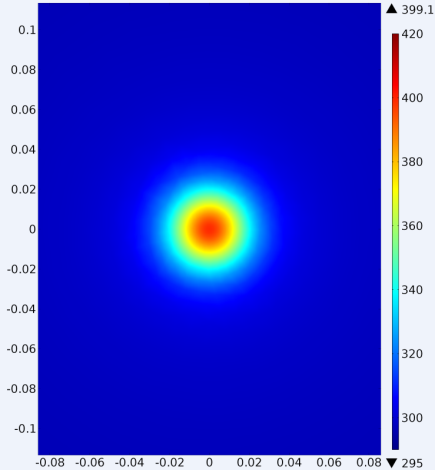
\includegraphics[width=0.3\linewidth]{fig2d.png}} \hfill
  \subfigure[]{\label{subfig:3b}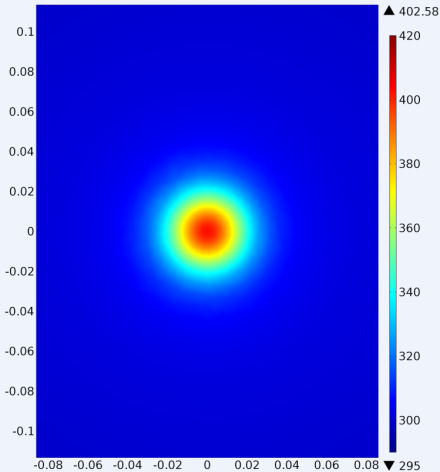
\includegraphics[width=0.3\linewidth]{fig2e.png}} 
  \subfigure[]{\label{subfig:3c}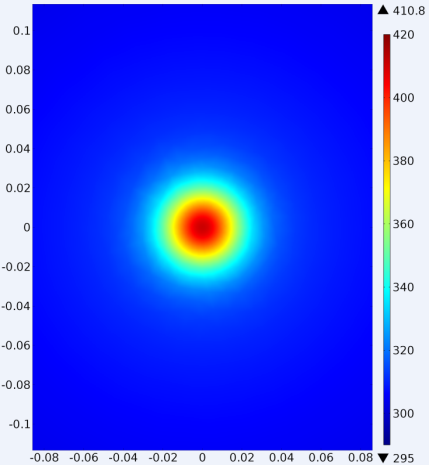
\includegraphics[width=0.3\linewidth]{fig2f.png}} 
	\hspace*{\fill} \\ \hspace*{\fill}
  \subfigure[]{\label{subfig:3d}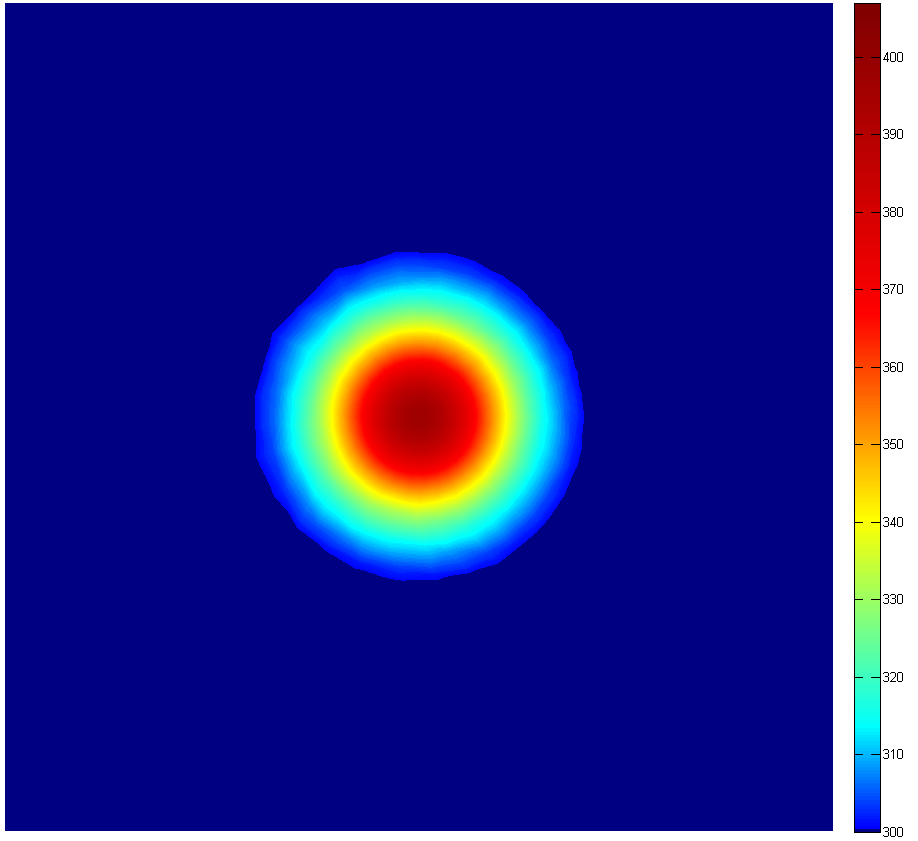
\includegraphics[width=0.3\linewidth]{1.png}} \hfill
  \subfigure[]{\label{subfig:3e}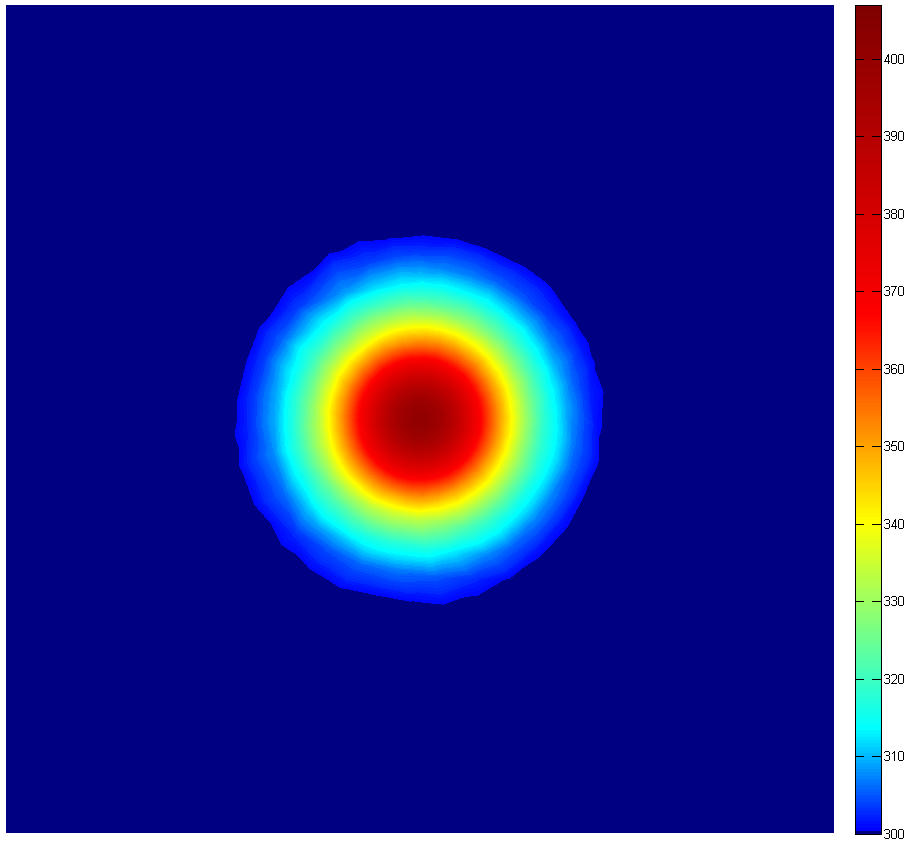
\includegraphics[width=0.3\linewidth]{2.png}} 
  \subfigure[]{\label{subfig:3f}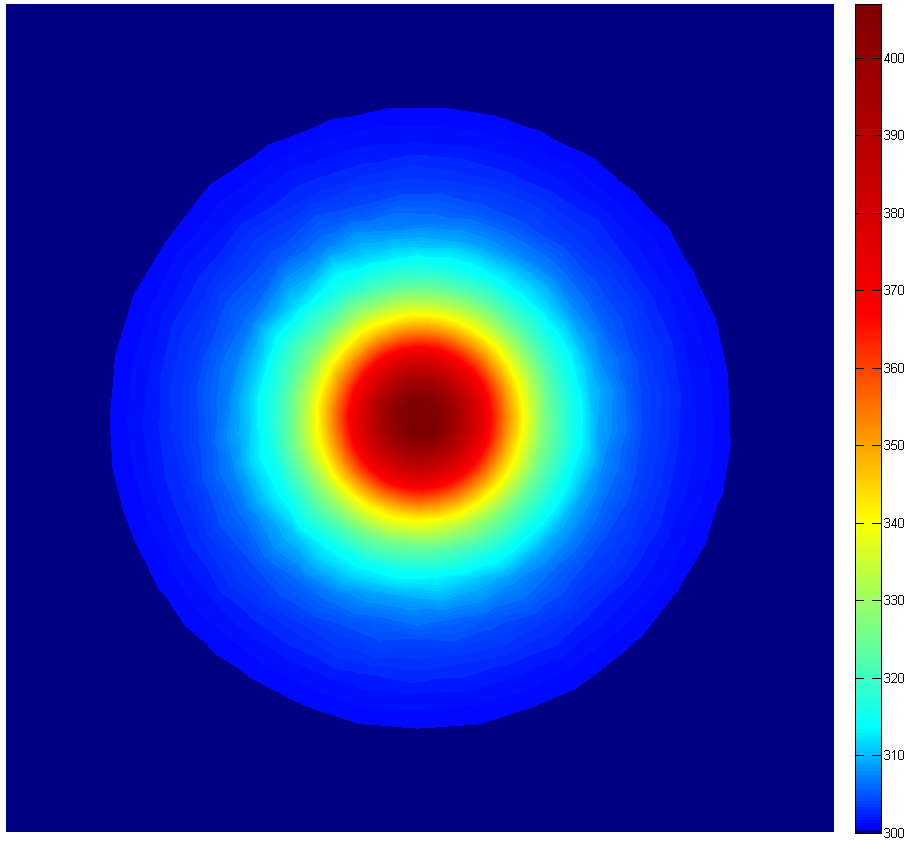
\includegraphics[width=0.3\linewidth]{3.png}} 
  \hspace*{\fill}
	
	  % \caption{(a) and (d) Thermal response, observed on a non-defective area - (b) and (e) 
	% Thermal response, observed on an area with defect of 1 mm below surface - (c) and (f) 
	% Thermal response, 
	% observed on an area with defect of 0.5 mm below surface.}
	
  % \label{fig:3}
\end{figure}

\end{document}
